% Sample LaTeX file for creating a paper in the Morgan Kaufmannn two
% column, 8 1/2 by 11 inch proceedings format.

\documentclass[]{article}
\usepackage{proceed2e}
\usepackage[
backend=bibtex,
style=alphabetic,
citestyle=authoryear
]{biblatex}
\usepackage{aliascnt}
\usepackage{amsmath}
\usepackage{amsfonts}
\usepackage{caption}
\usepackage{mathtools}
\usepackage[capitalise, noabbrev]{cleveref}
\usepackage{float}
\usepackage{algorithm}
\usepackage{algorithmic}
\usepackage{bbm}
\usepackage{amsthm}

% Set the typeface to Times Roman
\usepackage{times}


%\binoppenalty=\maxdimen % to prevent breaking equations
%\relpenalty=\maxdimen % to prevent breaking equations
% Define the equation float env
\newaliascnt{eqfloat}{equation}
\newfloat{eqfloat}{h}{eqflts}
\floatname{eqfloat}{Equation}


\newtheorem{proposition}{Proposition}

\title{Differentiable Particle Filter}

\author{} % LEAVE BLANK FOR ORIGINAL SUBMISSION.
          % UAI  reviewing is double-blind.

% The author names and affiliations should appear only in the accepted paper.
%
%\author{ {\bf Harry Q.~Bovik\thanks{Footnote for author to give an
%alternate address.}} \\
%Computer Science Dept. \\
%Cranberry University\\
%Pittsburgh, PA 15213 \\
%\And
%{\bf Coauthor}  \\
%Affiliation          \\
%Address \\
%\And
%{\bf Coauthor}   \\
%Affiliation \\
%Address    \\
%(if needed)\\
%}



\addbibresource{DPFbibli.bib}

\begin{document}

\maketitle

\begin{abstract}
	Sequential Monte Carlo (SMC or Particle Filters) methods are a set of powerful techniques for continuous state space models. Additionally to providing a belief for the state of an observed system, they also provide an estimate of its likelihood which is non-differentiable with respect to the model parameters. This is due to the fact that standard resampling schemes consist in a non-smooth re-indexing of the Monte Carlo sample. In this article we propose two new resampling schemes that rely on regularised optimal transport techniques and are respectively differentiable but biased, and non-differentiable but optimal in a certain metric. Furthermore we assess the behaviour of the methods in a linear setup by comparing with the Kalman Filter and discuss the influence of the hyper-parameters.
\end{abstract}

\section{INTRODUCTION}
	Particle Filters \parencite[see][]{particlefilter} offer an efficient way of performing posterior inference in otherwise intractable non-linear state space models and provide an unbiased estimate of the likelihood of the state space model parameters given observed data. Formally particle filters are interested in estimating state space hidden Markov models described by an unobserved state $X_t \in \mathbb{R}^{d_X}$ following $X_t|(X_{t-1}=x) \sim f_t(\cdot|x), t > 0$ and $X_0 \sim \mu(\cdot) \in \mathcal{M}(\mathbb{R}^{d_X})$ and an observed process $Y_t|(X_t=x) \sim g_t(\cdot|x) \in \mathcal{M}(\mathbb{R}^{d_Y})$. They do this by keeping track of $X_t$ in the form of a weighted sample $(w^i_t, X_t^i)$ through a method called Sequential Importance Sampling, however, this technique applied by itself leads to weight degeneracy that needs to be mitigated \parencite[see][]{doucet2009tutorial}, a well accepted way to fight this is through the use of a resampling scheme that replaces low weight particles with high weights ones \parencite[see][]{hol2006resampling}. 
	
	In this paper we focus on regularised optimal transport as a resampling technique in two different ways: in \cref{sec:differentiable} we use the planning matrix as a direct map from a weighted sample $(w_i, X_i) \sim \mathbf{X}$ to an equally weighted sample $(\mathbbm{1}_N, \mathbf{Z}_i^{\epsilon}) \sim \mathbf{X}^{\epsilon}$, where $\mathbbm{1}_N$ is the vector of size $N$ filled with $\frac 1 N$ and show $\mathbf{X}^{\epsilon} \xrightarrow[\epsilon \to 0]{\mathcal{L}} \mathbf{X}$, because the mapping we use is differentiable w.r.t $(w_i, X_i)$, it will provide a biased but differentiable resampling scheme, then in \cref{sec:optimal} we provide a novel algorithm that learns the optimal equally-weighted sample $(\mathbbm{1}_N, \mathbf{Z}_i^{\epsilon})$ in the $\epsilon$-Sinkhorn divergence sense. 
	
	
	Our main contributions are two fold: we introduce the planning matrix of the regularised optimal transport as a differentiable resampling scheme and we introduce a novel resampling algorithm that guarantees optimality of the resampled particles.
	
	The rest of the paper is organised as follows: in \cref{sec:background} we give a brief recapitulation of the Particle Filter \parencite[][]{particlefilter}, the biased Sinkhorn distances \parencite[][]{cuturi2013sinkhorn} and the Sinkhorn divergence \parencite[][]{feydy:interpolating}, in \cref{sec:differentiable} we introduce the differentiable particle filter, discuss its behaviour and provide examples, in \cref{sec:optimal} we introduce an optimal resampling scheme and provide examples for it, and finally we conclude with future possible extensions and improvements.

\section{BACKGROUND}
\label{sec:background}
	\subsection{Particle Filters}
	\label{subsec:PF}
	 	
		Particle filters have emerged as a standard technique for non linear data assimilation and approximates the filtering (posterior) distribution $X_t|(Y_t=y, X_{t-1}))$ using a weighted set of $N$ samples $(w_i, X_i)$ which are updated following a predict-update approach. Any given quantity of interest $\mathbb{E}[\phi(X_t)]|(Y_t=y, X_{t-1}))]$ can then estimated as a weighted average $\sum_i w_i \phi(X_i)$ with variance given by a central limit theorem \parencite[see][]{chopin2004central}. 
		The "predict step" consists in proposing particles $X_t^i \sim p(\cdot|\mathbf{X}_{t-1}=X_{t-1}^i)$ whose weights will then be updated as per the bayes formula: 
		
		\begin{align}
			w_t^i &= p(X_t^i|\mathbf{Y}_t=\mathbf{y},X_{t-1}^i) \\
			&\propto p(Y_t|X_{t}^i) \cdot p(X_t^i|X_{t-1}^i) \label{eq:likelihood}\\
			&= p(Y_t|X_{t}^i) \cdot w_{t-1}^i
		\end{align}
	
		
		These will then be normalised to sum to 1. Additionally the marginal likelihood $P(\mathbf{Y}_{u=1..t}|\mathbf{X}_{u=1..t}, \mathbf{\theta})$ up to time time $T$ where $\mathbf{\theta}$ are model parameters can be estimated through \cref{eq:likelihood} prior to normalisation.
		
		However, as time passes, the weights suffer a well-known degeneracy problem, that is all weights will converge to 0 apart from 1, hence not providing a good distributional estimate for the posterior. This has traditionally been mitigated by ancestry resampling: instead of proposing $X_t^i \sim p(\cdot|\mathbf{X}_{t-1}=X_{t-1}^i)$, we propose $X_t^i \sim p(\cdot|\mathbf{X}_{t-1}=X_{t-1}^{a_i})$ where $a_i \in {1,..,N}$ is any index sampling such that $\mathbb{E}[\sum_i \mathbb{I}(a_i=j)|\mathbf{w}] = N w_j, \, \forall j \in {1,...,N}$ \parencite[see][]{doucet2009tutorial}. In practice this is only done when the efficient sample size (ESS) $\frac{1}{\sum_i w_i^2}$ is lower than a certain threshold (usually 50\% of the sample size $N$).
		
		This is summarised in \cref{algo:bootstrap} and \cref{algo:resampling}. Because of the reparametrization trick \parencite[see][]{kingma2013auto}, only \cref{algo:resampling} makes the particle filter non-differentiable with respect to its inputs.
		
		\begin{algorithm}
			\caption{Bootstrap Particle Filter}
			\label{algo:bootstrap}
			\begin{algorithmic}
				\STATE{\bfseries Input:} $X_i$, $w_i$, $y$, $N$, $X$, $L$ \COMMENT{Inputs at time $t > 0$}, 
				\IF{$\text{ESS} < N \cdot \text{threshold}$}
					\STATE{Resample}
				\ENDIF
				\FOR{$i=1$ {\bfseries to} $N$}
					\STATE{Propose:} Sample $X_i ~ p(X_{t+1}|X_t=X_i)$
					\STATE{Update:} Compute $w_i *= p(Y_t=y|X_t=X_i)$
				\ENDFOR
				\STATE{Compute log-likelihood update:} $L+=\log{\sum_i w_i}$
	
				\FOR{$i=1$ {\bfseries to} $N$}
					\STATE $w_i = \frac{w_i}{\sum_i w_i}$
				\ENDFOR
			\end{algorithmic}
		\end{algorithm}
	
		\begin{algorithm}
			\caption{Generic resampling}
			\label{algo:resampling}
			\begin{algorithmic}
				\STATE{\bfseries Input:} $X_i$, $w_i$, $N$,
				\FOR{$i=1$ {\bfseries to} $N$}
					\STATE{Sample:} $a_i$ \COMMENT{satisfying hypotheses, for example $a_i \sim \text{Multinomial}(\mathbf{w})$} 
					\STATE{Set:} $w_i = \frac{1}{N}$, $X_i = X_{a_i}$
				\ENDFOR
				\OUTPUT $\mathbf{w}$, $\mathbf{X}$ 
			\end{algorithmic}
		\end{algorithm}

	In this article, similarly to \parencite{reich2012nonparametric,graham2019scalable} we consider an ensemble approach to particle filtering: instead of the resampling scheme $(w_i, X_i) \mapsto (\frac 1 N, X_{a_i})$ we provide two new mappings: we present a biased ensemble reweighting (\cref{sec:differentiable}) that comes from the planning matrix solution of a regularised Optimal Transport problem $(w_i, X_i) \mapsto (\frac 1 N, (M_{\epsilon}^{\mathbf{w}, \mathbf{X}} X)_i)$, and we present a learnt optimal recentering of the particles learnt to minimize the Sinkhorn Divergence \parencite[see][]{genevay2017learning,feydy:interpolating} $(w_i, X_i) \mapsto (\frac 1 N, Z^{\epsilon}_i)$.

	\subsection{REGULARISED OPTIMAL TRANSPORT}
	\label{subsec:OT}
		\subsubsection{Optimal Transport}
			Optimal transport is interested in computing a distance between measures. Formally, given two empirical probability measures $\alpha, \beta \in \mathcal{M}^+_1(\mathcal{X})$, and given a symmetric positive cost function $C: \mathcal{X} \times \mathcal{X} \to \mathbb{R}$, it is interested in computing both the minimum and the minimising argument of the functional $\pi \mapsto \int_{\mathcal{X}^2} C(x,y) d \pi$ for $\pi$ belonging to the simplex 
			$$S_{\alpha, \beta} = \left\{ \pi \in \mathcal{M}^+_1(\mathcal{X} \times \mathcal{X} ) | \int \pi(\cdot, dy) = \alpha, \int \pi(dx, \cdot) = \beta \right\}$$
			
		\subsubsection{Sinkhorn distances}
		
			If the supports of $\alpha$ and $\beta$ are of size $N$, this is known to scale in $O(n^3)$. \cite{cuturi2013sinkhorn} shows that a regularised version of the algorithm can be considered instead:
			$$\textbf{OT}_{\epsilon} := \min_{\pi \in S_{\alpha, \beta}} \int_{\mathcal{X}^2} C(x,y) d \pi + \epsilon KL(\pi||\alpha \otimes \beta)$$
			
			Thanks to Fenchel-Rockafellar theorem, this can be rewritten \parencite[see][]{feydy:interpolating,peyr2018computational} using dual functions $f, g \in \mathcal{C}(\mathcal{X})$:
			\begin{align}
				\textbf{OT}_{\epsilon} 	=&\max_{f, g \in \mathcal{C}(\mathcal{X})} \langle \alpha, f \rangle + \langle \beta, g \rangle \\
										&- \epsilon \langle \alpha \otimes \beta, \exp \left( \frac 1 \epsilon \left( f \oplus g - C \right)  \right) - 1 \rangle \nonumber\\
				\text{with: } \pi_{\epsilon} 			= &\exp \left( \frac 1 \epsilon \left( f \oplus g - C \right)  \right) \cdot \alpha \otimes \beta \label{eq:plan}
			\end{align}
			
			This has been key for the recent development of computational optimal transport \parencite{peyr2018computational} as it translates a problem over a matrix to a problem over two related vectors. Moreover the optimality condition on $f$ and $g$ can be written in a fixed-point theorem form: if $\alpha = (w^X_i, X_i)_{1 \leq i \leq N}, \beta = (w^Y_j, Y_j)_{1 \leq j \leq M}$ \parencite{feydy:interpolating} which one only has to iterate successively to until convergence.
			
			\begin{align}
				\forall i, j &\nonumber\\
				f_i &= -\epsilon \text{LSE}_k(\log w^Y_k + \frac 1 \epsilon g_k - \frac 1 \epsilon C(X_i, Y_k)) \label{eq:fixed_1}\\
				g_j &= -\epsilon \text{LSE}_k(\log w^X_k + \frac 1 \epsilon f_k - \frac 1 \epsilon C(X_k, Y_j)) \label{eq:fixed_2}
			\end{align}
			
	
		\subsubsection{Sinkhorn divergences}
			\label{subsubsec:Div}
			Crucially $\textbf{OT}_{\epsilon}(\cdot, \alpha)$ doesn't reach its minimum in $\alpha$, which means that the solution of $\min_{\beta} \textbf{OT}_{\epsilon}(\beta, \alpha)$ may actually lay far from $\alpha$. This has been outlined first in \cite{genevay2017learning}, and a solution is to consider instead the so-called "Sinkhorn Divergence" 
			\begin{align}
				\mathcal{W}_\epsilon(w_X, X, w_y, Y) := 
					& \; \text{OT}_{\epsilon}(w_X, X, w_y, Y) \label{eq:non_sym}\\
					& - 0.5 \text{OT}_{\epsilon}(w_X, X, w_X, X) \label{eq:sym_1}\\
					& - 0.5 \text{OT}_{\epsilon}(w_Y, Y, w_Y, Y)\label{eq:sym_2}
			\end{align}
			
			An important point is that the symmetric Optimal transport problems \cref{eq:sym_1,eq:sym_2} can be solved faster than the non-symmetric one, hence the computational burden is controlled by \cref{eq:non_sym}

\section{DIFFERENTIABLE RESAMPLING}
\label{sec:differentiable}
	Given a weighted empirical distribution $(w_i, X_i)_{1 \leq i \leq N} \in \mathcal{M}^+_1(\mathbb{R}^d$ we are interested in finding a "good enough" unweighted sample in the sense that for any $\phi := \mathbb{R}^d \to \mathbb{R}$, $\sum_{1 \leq i \leq N} w_i \phi(X_i) \approx \frac{1}{N}\sum_{1 \leq i \leq N} \phi(X_i)$ with small enough variance \parencite[][]{resampling_comp}. While most approaches consider a bootstrapping of the particle based on the weights: $(w_i, X_i) \mapsto (\frac 1 N, X_{a_i})$ this provides a non-differentiable mapping that prevents exact propagation of the gradient through the resampling step. Because of this and to prevent high variance in the gradient estimation, recent works by \cite{maddison2017filtering,naesseth2017variational,le2017auto} that link SMC and Variational Inference simply ignore the additional impact of resampling and tweak the AutoDiff scheme to propagate the gradient of particles that were not discarded at the resampling step only. As discussed in their papers this provides a biased estimator of the likelihood.
	
	\subsection{OPTIMAL TRANSPORT MAP RESAMPLING}
	\label{subsec:otResampling}
		To the best of our knowledge the first paper to have introduced Optimal Transport map as an ensemble technique for resampling is \cite{reich2012nonparametric}, and the method has since been applied in \cite{graham2019scalable} and \cite{jacob2016coupling} to provide a local mapping from prior to posterior and to couple same-seed particle filters trajectories in order to compute sensitivities with respect to its hyper-parameters. 
		
		The paradigm introduced in \cite{reich2012nonparametric} can be phrased as follows.
		Let $(w, X)_i$ be a weighted sample before resampling and $C \in \mathbb{R}^d \times \mathbb{R}^d$ be a symmetric positive cost matrix, and lets consider the following Optimal Transport problem: 
		\begin{align}
			\mathbf{U} = \text{argmin}_{M \in S_{\mathbf{w}, \mathbf{1}_N}} \sum_{i,j} C_{i,j}, M_{i,j} \label{eq:ot_res}
		\end{align}
		
		As discussed in	\cite{reich2012nonparametric}, this matrix constitutes a Markov Chain $\mathbf{P} := N \mathbf{U}$ and the mapping $\tilde{X} = \mathbf{P} \mathbf{X}$ provides a consistent estimate of $(w_i, X_i)_i$.
		
		However the function $(w_i, X_i)_i \to \mathbf{P}\mathbf{X}$ is difficult to compute \parencite[see][]{cuturi2013sinkhorn}.
		
	\subsection{DIFFERENTIABLE RESAMPLING}
	\label{subsec:regOTResamp}
		Instead of considering the non-regularised problem in \cref{eq:ot_res}, we instead use the mapping resulting from the regularised version of the Optimal Transport problem \cref{eq:plan} \parencite{cuturi2013sinkhorn,feydy:interpolating} $(\mathbf{w}, \mathbf{X}) \to \mathbf{P}_\epsilon \mathbf{X}$.
		
		\begin{proposition}
			\label{prop:differentiability}
			The mapping $$(\mathbf{w}, \mathbf{X}) \to \mathbf{P}_\epsilon = \exp \left( \frac 1 \epsilon \left( \mathbf{f}^T + \mathbf{g} - \mathbf{C}(\mathbf{X},\mathbf{X}) \right)  \right) \cdot \mathbf{w}^T$$ where $\mathbf{f}$ and $\mathbf{g}$ are given by \cref{eq:fixed_1,eq:fixed_2} is differentiable, with:
			\begin{align}
				\forall i, j &\nonumber\\
				\frac{\partial f_i}{\partial \cdot} &= \frac{\partial}{\partial \cdot}-\epsilon \text{LSE}_k(\log w^Y_k + \frac 1 \epsilon g_k - \frac 1 \epsilon C(X_i, Y_k)) \label{eq:fixed_1_deriv}\\
				\frac{\partial g_j}{\partial \cdot} &= \frac{\partial}{\partial \cdot}-\epsilon \text{LSE}_k(\log w^X_k + \frac 1 \epsilon f_k - \frac 1 \epsilon C(X_k, Y_j)) \label{eq:fixed_2_deriv}
			\end{align}
		\end{proposition}
	
		\begin{proof}
			The system of equations \cref{eq:fixed_1,eq:fixed_2} defines an system of implicit functions to which we can apply the implicit function theorem. In this case the application of it is trivial as the relationship is linear.
		\end{proof}
	
		In practice this means that the gradients can be propagated by automatic differentiation at the last step of the Sinkhorn iterates only provided that the algorithm has converged. 
		
		When using automatic differentiation, this can be summarised as:
		\begin{algorithm}
			\caption{Biased resampling}
			\label{algo:biasedResampling}
			\begin{algorithmic}
				\STATE{\bfseries Input:} $X_i$, $w_i$, $N$, $n_{\text{steps}}$
				\STATE Stop registering gradients
				\STATE{\bfseries Initialise:} $\mathbf{f}$, $\mathbf{g}$
				\STATE 
					\FOR{$i=1$ {\bfseries to} $n_{\text{steps}}-1$}
						\STATE evaluate \cref{eq:fixed_1} and \cref{eq:fixed_2} simultaneously
					\ENDFOR
				\STATE Register gradients
				\STATE Set gradients of $\mathbf{f}$, $\mathbf{g}$ to $0$
				\STATE Evaluate \cref{eq:fixed_1}, \cref{eq:fixed_2}
				\OUTPUT $\frac 1 N \mathbbm{1}_N$, $\mathbf{P} \mathbf{X}$ with $P$ given by \cref{eq:plan}
			\end{algorithmic}
		\end{algorithm}
		
		
		
		\subsubsection{Illustration}
			To illustrate the behaviour of the resampling scheme we consider a bimodal 2D distribution of 500 constructed as follows: 500 points $X_i \in \mathbb{R}^2$ are drawn uniformly within a circle of radius 1, then half the sample is randomly set to have weights proportional to $\mathcal{N}\left(\left(\begin{matrix}-0.5 \\ 0.5\end{matrix}\right), \left(\begin{matrix}0.3 & 0.\\ 0. & 0.3 \end{matrix}\right)\right)$ and the other half $\mathcal{N}\left(\begin{matrix}0.5 \\ -0.5\end{matrix}, \begin{matrix}0.1 & 0.\\ 0. & 0.1 \end{matrix}\right)$, see \cref{fig:BiasedTransport}. This corresponds tp a multimodal distribution $X |\, ||X||^2_2 \leq 1$ where $X\sim \mathcal{N}\left(\left(\begin{matrix}-0.5 \\ 0.5\end{matrix}\right), \left(\begin{matrix}0.3 & 0.\\ 0. & 0.3 \end{matrix}\right)\right) + \mathcal{N}\left(\left(\begin{matrix}0.5 \\ -0.5\end{matrix}\right), \left(\begin{matrix}0.1 & 0.\\ 0. & 0.1 \end{matrix}\right)\right)$
			
			\begin{figure}
				\centering
				\captionsetup{justification=centering}
				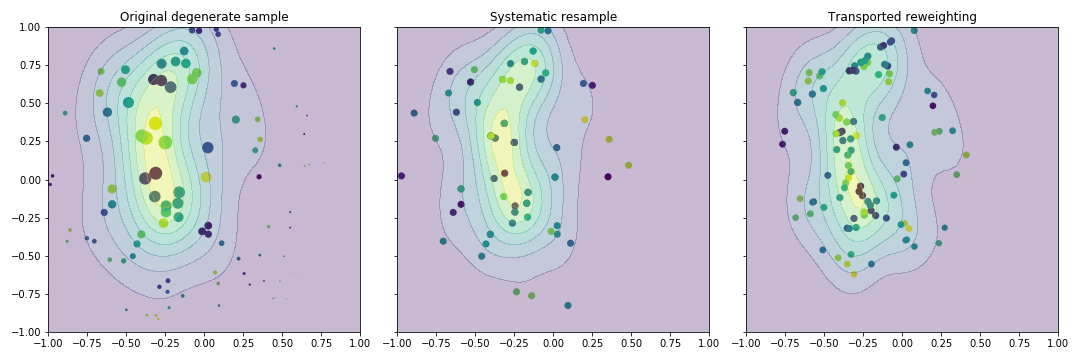
\includegraphics[width=\linewidth]{BiasedTransport}
				\caption{Biased transport comparison}
				\label{fig:BiasedTransport}
			\end{figure}	
		
			\cref{fig:BiasedTransport} illustrates a well-known problem of the regularised Sinkhorn algorithm: as the regularisation increases, the resulting transporting plan will converge to the one that minimizes $KL(\pi||\alpha\otimes\beta)$, in this case $\mathbf{w_X} \otimes \mathbf{\mathbbm{1}_N}$, hence the resulting resampling of $\mathbf{X}$: $\mathbf{X_\epsilon} = \mathbf{P_\epsilon} \mathbf{X}$ collapses to the weighted mean of the sample $\mathbf{X}$.
			
		\subsubsection{Application To A State Space Model}
			We now consider the following noisy resonator:
			
			\begin{align}
				x_\text{true}(t) = \sin(t) + \frac 1 2 \mathcal{N}(0, 1), t = 0., 0.1, ..., 20
			\end{align}
			
			That we model by the following 2D state space model

			\begin{align}
				\label{eq:ssm}
				x_0(t + dt) &= x_0(t) + x_1(t) dt + N(0, \sigma_0^2)\\				
				x_1(t + dt) &= x_1(t) - x_0(t) dt + N(0, \sigma_1^2)\\
				y(t) &= x_0(t) + N(0, \sigma_y^2)
			\end{align}
			
			\begin{figure}
				\centering
				\captionsetup{justification=centering}
				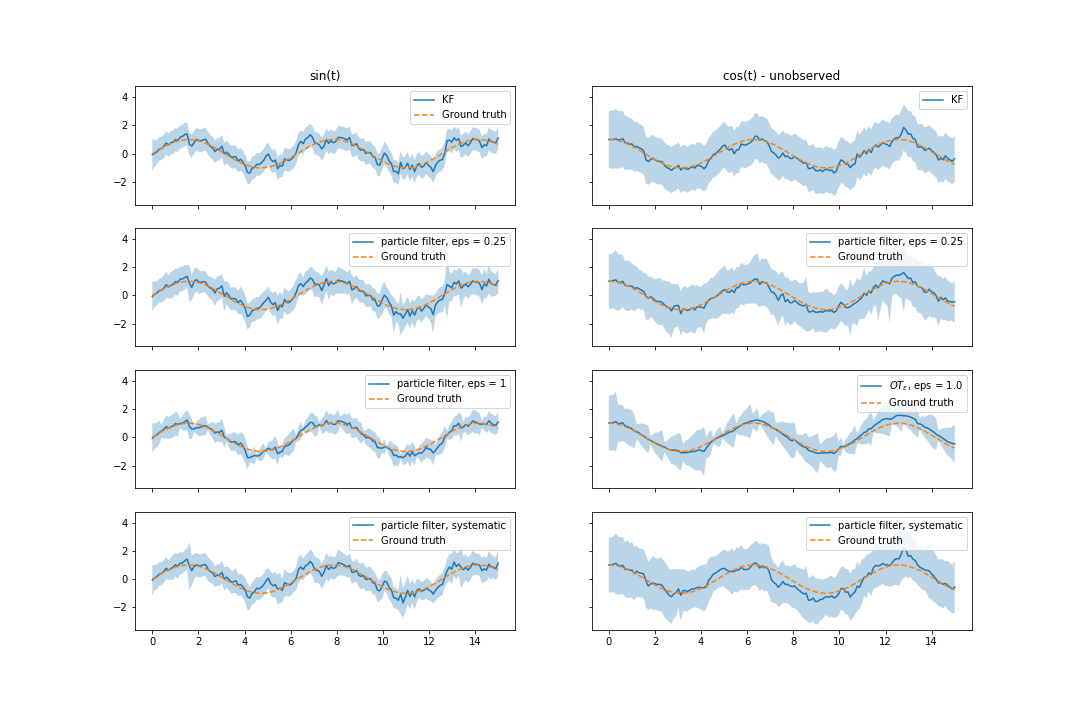
\includegraphics[width=\linewidth]{KF_OptimalTransportPF_comp}
				\caption{Filtering applied to \cref{eq:ssm}
				Top: Kalman Filter, Second and Third: Biased Transport with $\epsilon=0.25,1$, Bottom: Systematic Resampling }
				\label{fig:kf_illustration}
			\end{figure}	
		
			\cref{fig:kf_illustration} compares \cref{algo:biasedResampling} for different regularisations with \cref{algo:resampling} with systematic resampling \parencite{resampling_comp}, all filters have 100 particles. The shaded zone corresponds to $\pm 2 \text{standard deviations}$ 
			
			The collapsing phenomenon in the sample due to the regularisation as highlighted in \cref{fig:BiasedTransport} is visible in \cref{fig:kf_illustration}: each resampling step results in a decrease in variance of the sample.
			
		\subsubsection{Likelihood evaluation}
			Together with the resampling in \cref{algo:resampling} the formula coming from \cref{algo:bootstrap} provides an unbiased estimate of the likelihood for the state space model associated and also comes with a central limit theorem \cite{chopin2004central}. However, the resulting function $\hat{\mathcal{L}}(\mathbf{y}|\mathbf{\theta})$ is not continuous and as a consequence not differentiable with respect to $\mathbf{\theta}$. On the other hand using \cref{algo:biasedResampling} provides a theoretically everywhere differentiable scheme for "recentering" the particles, albeit to the cost of biasedness in the resulting estimate.
			
			
			\begin{figure*}
				\centering
				\captionsetup{justification=centering}
				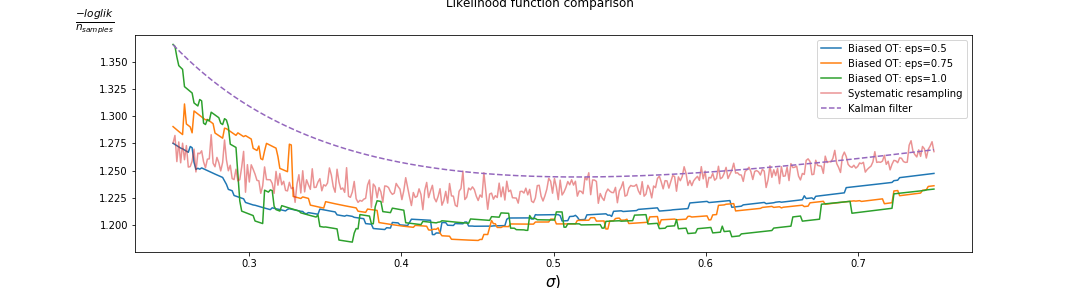
\includegraphics[width=\textwidth]{likelihood}
				\caption{Likelihood estimate w.r.t. the observation log-error, 400 points}
				\label{fig:likelihood}
			\end{figure*}
			
			\begin{figure*}
				\centering
				\captionsetup{justification=centering}
				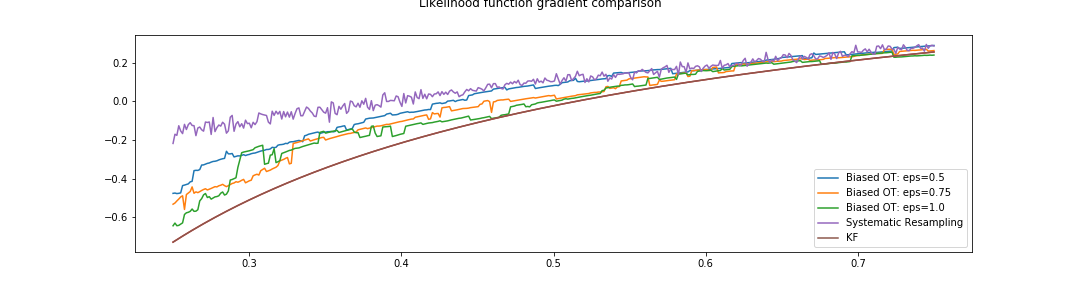
\includegraphics[width=\textwidth]{likelihoodGradient}
				\caption{Gradient of the likelihood estimate w.r.t. the observation log-error}
				\label{fig:likelihoodGradient}
			\end{figure*}
			

\section{OPTIMAL RESAMPLING}
\label{sec:optimal}

	While the scheme in \cref{sec:differentiable} has the advantage of providing a gradient for the resampling schemes, it suffers from the inconvenient of providing a collapsed estimate of the state post resampling, which in turns results in a biased estimate of the likelihood. Instead of learning a biased linear mapping, we can instead learn the best unweighted point cloud minimising a distance from the weighted degenerate sample. To this end we consider the Sinkhorn divergence (see \cref{subsubsec:Div})
	
	\subsection{LEARNT POINTS CLOUD}
		As in \cite{genevay2017learning} we consider the optimisation problem given by the Wasserstein divergence $\mathcal{W}_\epsilon = 2 OT_{\epsilon}(\alpha,\beta) - OT_{\epsilon}(\alpha,\alpha) - OT_{\epsilon}(\beta,\beta)$, where in our case $\alpha$ is the weighted degenerate sample $(w_i, X_i)_i$ and $\beta$ is the target unweighted sample $(\frac 1 N, Z_i)_i$: this constitutes a gradient descent on $Z$ with respect to the loss given by the Wasserstein divergence.
		
		The resampling algorithm is therefore modified as in \cref{algo:optimalResampling}
		
		\begin{algorithm}
			\caption{Optimal resampling}
			\label{algo:optimalResampling}
			\begin{algorithmic}
				\STATE{\bfseries Input:} $X_i$, $w_i$, $N$, $n_{\text{steps}}$, tolerance, $\lambda$ \COMMENT{Learning rate}
				\STATE Stop registering gradients
				\STATE{\bfseries Initialise:} $\mathbf{f}$, $\mathbf{g}$
				\STATE $Z \leftarrow X$
				\FOR{$i=1$ {\bfseries to} $n_{\text{steps}}$}
					\IF{$\mathcal{W}_\epsilon(w,X,\frac 1 N, Z)<\text{tolerance}$}
						\STATE Break
					\ENDIF
					\STATE $Z \leftarrow Z - \lambda \nabla_Z \mathcal{W}_\epsilon$
				\ENDFOR
				\OUTPUT $\frac 1 N \mathbbm{1}_N$, $Z$
			\end{algorithmic}
		\end{algorithm}
		
		\begin{figure*}
			\centering
			\captionsetup{justification=centering}
			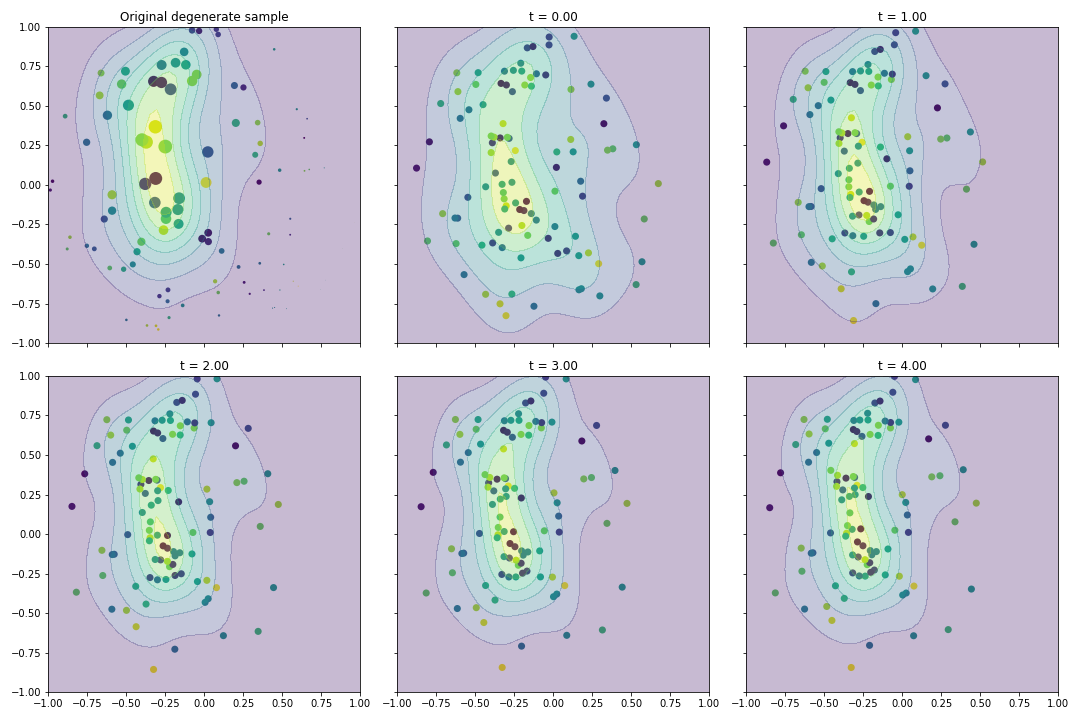
\includegraphics[width=\textwidth]{LearntReweighting}
			\caption{Gradient Flow for learning the unweighted sample\\
				Top left: original sample, right and bottom: evolution of the gradient descent}
			\label{fig:LearntReweighting}
		\end{figure*}	

		
		The behaviour of \cref{algo:optimalResampling} is shown in \cref{fig:LearntReweighting}
	


\section{CONCLUSION AND FUTURE WORKS}
\label{sec:conclusion}



\subsubsection*{References}

\printbibliography[heading=none]


\end{document}
